\documentclass{article}

\usepackage{fontspec}
\setmainfont{Libertinus Serif}
\usepackage[margin=1in]{geometry}

\usepackage{tikz}
\usetikzlibrary{arrows.meta}
\usetikzlibrary{positioning}
\usetikzlibrary{quotes}

\input plaincenter
\parindent=0pt

\def\chapelmaster#1#2#3{%
    \vbox{\hsize=0.33\hsize
    \begcenter
    #1\par
    #2\par
    #3\par
    \endcenter
    }%
}
\def\job#1#2{%
    #1\hfil#2\par
}
\def\Fernandez{%
    \chapelmaster
    {Gaspar Fernández}
    {(15xx--1628)}
    {\job{16xx--1628}{MC Puebla Cat.}}%
}
\def\Padilla{%
    \chapelmaster
    {Juan Gutiérrez de Padilla}
    {(1590--1664)}
    {\job{16xx--1622}{MC Cádiz Cat.}%
     \job{1628--1664}{MC Puebla Cat.}}%
}
% \def\Garcia{García de Céspedes}
% \def\Vidales{Vidales}
% \def\Vasquez{Vásquez}
% \def\Santiago{Santiago}
% \def\Lobo{Lobo}
% \def\Dupont{Dupont}
% \def\Jalon{Jalón}

\begin{document}
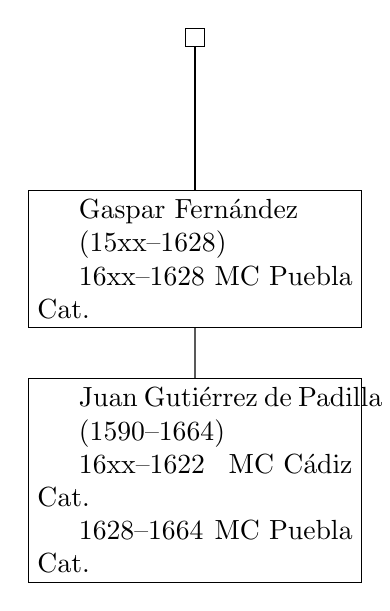
\begin{tikzpicture}[every node/.style={draw},
    level distance=8em]
    \node (root) {}
        child { node (p1) {\Fernandez} 
            child { node (p2) {\Padilla} 
            }
        };
\end{tikzpicture}
\end{document}

